\documentclass[11pt]{article}

\usepackage[a4paper,margin=2.5cm]{geometry}
\usepackage{graphicx}
\usepackage{float}
\usepackage{amsmath,amssymb}
\usepackage{siunitx}
\usepackage{booktabs}
\usepackage{multirow}
\usepackage{caption}
\usepackage{subcaption}
\usepackage[round]{natbib}
\usepackage[hidelinks]{hyperref}

%% Number figures and tables as S1, S2, ... to mark them as supplementary.
\renewcommand{\thefigure}{S\arabic{figure}}
\renewcommand{\thetable}{S\arabic{table}}

\title{Online Resource 1\\[0.3em]
\large Supplementary figures and tables}
\author{}
\date{}

\begin{document}
\maketitle

\noindent
\textbf{Article:} \emph{Adult neurogenesis promotes pattern separation and sparsity beyond the dentate gyrus in a spiking
DG--CA3 model}\\[0.2em]
\textbf{Journal:} Cognitive Neurodynamics\\[0.2em]
\textbf{Authors:} Marlon Valmórbida Cendron, Wilfredo Blanco Figuerola, Flávio Freitas Barbosa\\[0.2em]

\textbf{Corresponding author:} Marlon Valmórbida Cendron, Laboratory for Memory and Cognition Studies, Department of Psychology,
Federal University of Paraíba, João Pessoa, Brazil. E-mail: marlonvcendron@gmail.com

\bigskip

%% =====================================================================
%% Table S1 -- in vivo firing rates and population sparsity
%% =====================================================================
\begin{table}[h!]
\centering
\renewcommand{\arraystretch}{1.4}
\resizebox{\textwidth}{!}{%
\begin{tabular}{lllllll}
\toprule
\textbf{Cell}
  & \textbf{\textit{In Vivo} Firing Rate (Hz)} & \textbf{Reference}
  & \textbf{Model Firing Rate (Hz)}
  & \textbf{\textit{In Vivo} Activation} & \textbf{Reference}
  & \textbf{Model Activation} \\
\midrule


\multirow[t]{7}{*}{$\vcenter{\hbox{
\includegraphics[height=1.5em]{mgc.png}}}$ Mature granule}
  & 1.2 (0.56--2.38)                        & \citet{mchughAdultborn2022}
  & \multirow[t]{7}{*}{1.08}
  & 2--5\%                                  & \citet{galloniRecurrent2022, hainmuellerParallel2018}
  & \multirow[t]{7}{*}{8.0\%} \\
  & 0.49                                    & \citet{diamantakiSparse2016}
  &
  & 9\%                                     & \citet{goodsmithSpatial2017}
  & \\
  & $0.031 \pm 0.096$                       & \citet{zhangSelective2020}
  & & & & \\
  & 0.4                                     & \citet{wheelerHippocampomeorg2023}
  & & & & \\
  & $0.96 \pm 0.19$                         & \citet{goodsmithDentate2019}
  & & & & \\
  & $\approx 0.2$                           & \citet{senzaiExtracellular2016}
  & & & & \\
  & $72 \pm 8$\textsuperscript{max}         & \citet{lubkeSpecialized1998}
  & & & & \\
\midrule


$\vcenter{\hbox{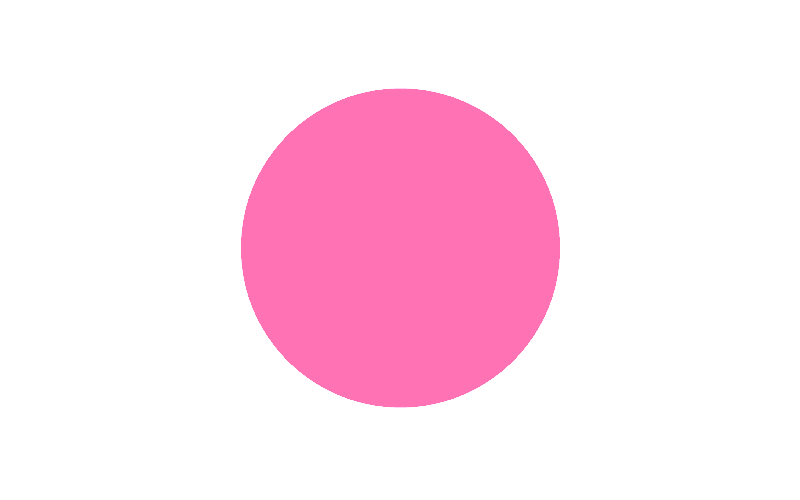
\includegraphics[height=1.5em]{igc.png}}}$ Immature granule
  & 2.3 (1.6--6.7)                          & \citet{mchughAdultborn2022}
  & 2.96
  &                                         &
  & 63.8\% \\
\midrule


\multirow[t]{4}{*}{$\vcenter{\hbox{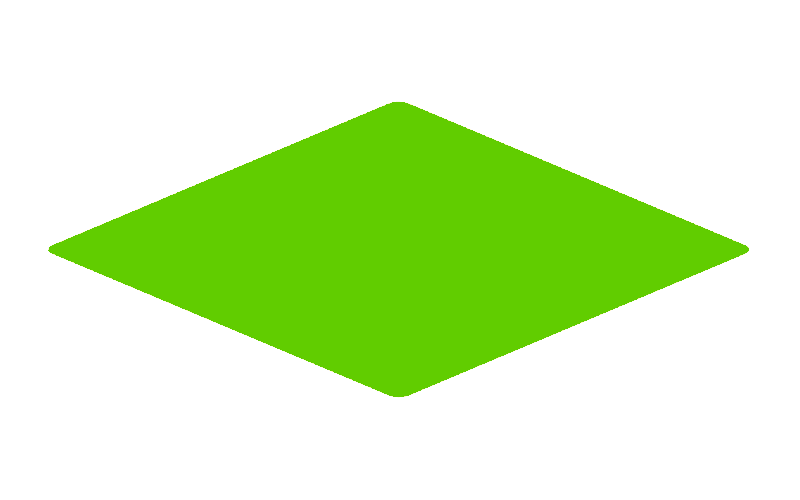
\includegraphics[height=1.5em]{mc.png}}}$ Mossy}
  & 0.84                                    & \citet{wheelerHippocampomeorg2023}
  & \multirow[t]{4}{*}{3.45}
  & $\approx 100\%$                         & \citet{danielsonVivo2017}
  & \multirow[t]{4}{*}{96.7\%} \\
  & $1.05 \pm 0.07$                         & \citet{goodsmithDentate2019}
  &
  & 88\%                                    & \citet{goodsmithSpatial2017}
  & \\
  & $\approx 0.8$                           & \citet{senzaiExtracellular2016}
  & & & & \\
  & $50 \pm 6$\textsuperscript{max}         & \citet{lubkeSpecialized1998}
  & & & & \\
\midrule

$\vcenter{\hbox{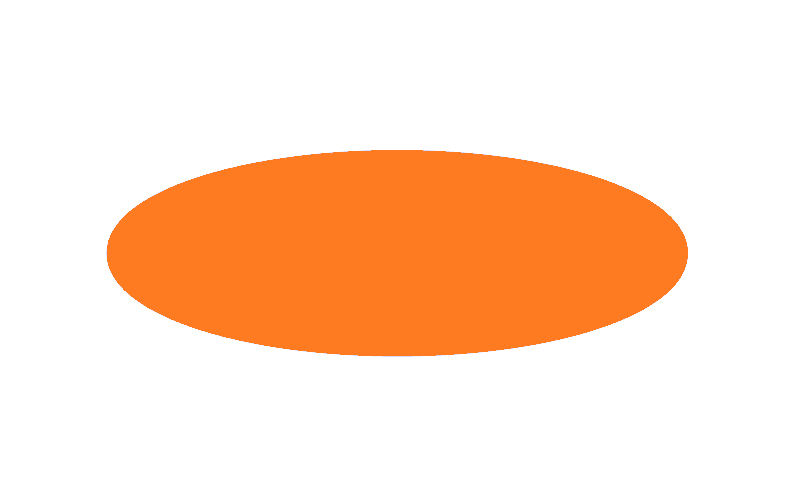
\includegraphics[height=1.5em]{hipp.png}}}$ HIPP
  & $111.4 \pm 10.2$\textsuperscript{max}   & \citet{yuanSomatostatinpositive2017}
  & 6.38
  &                                         &
  & 100\% \\
\midrule

\multirow[t]{2}{*}{$\vcenter{\hbox{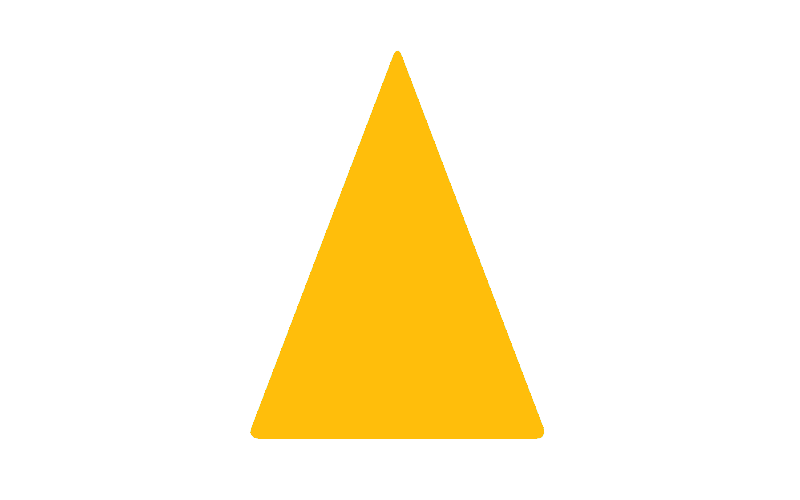
\includegraphics[height=1.5em]{bc.png}}}$ Basket}
  & $13.6 \pm 0.8$                          & \citet{liSustained2022}
  & \multirow[t]{2}{*}{17.35}
  &                                         &
  & \multirow[t]{2}{*}{100\%} \\
  & $230 \pm 15$\textsuperscript{max}       & \citet{lubkeSpecialized1998}
  & & & & \\
\midrule


\multirow[t]{7}{*}{$\vcenter{\hbox{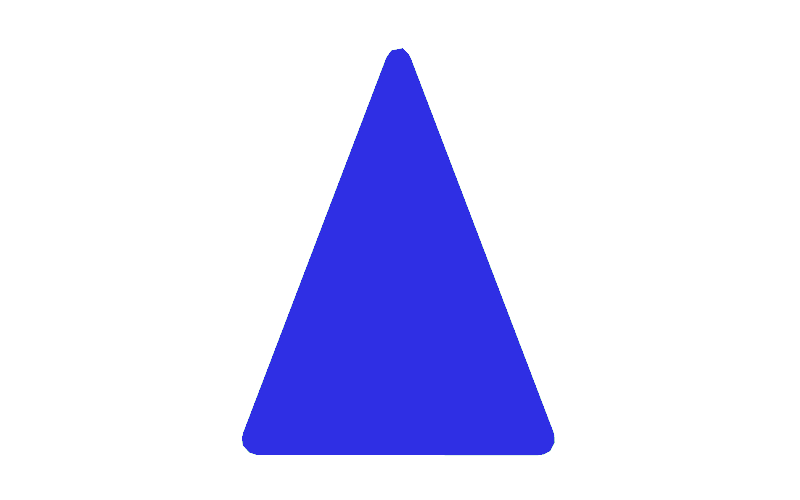
\includegraphics[height=1.5em]{pca3.png}}}$ CA3 pyramidal}
  & 0.2                                     & \citet{mizusekiPreconfigured2013}
  & \multirow[t]{7}{*}{1.17}
  & 29\%                                    & \citet{goodsmithSpatial2017}
  & \multirow[t]{7}{*}{30.0\%} \\
  & 0.5                                     & \citet{kayHippocampal2016}
  &
  & 20--30\%                                & \citet{galloniRecurrent2022}
  & \\
  & $0.72 \pm 0.51$                         & \citet{lasztocziTerminal2011}
  & & & & \\
  & CA3a: 0.4; CA3b: 0.3                    & \citet{olivaRole2016}
  & & & & \\
  & 1.2                                     & \citet{mchughAdultborn2022}
  & & & & \\
  & $0.92 \pm 0.06$                         & \citet{goodsmithDentate2019}
  & & & & \\
  & $\approx 0.6$                           & \citet{senzaiExtracellular2016}
  & & & & \\
\midrule


\multirow[t]{3}{*}{$\vcenter{\hbox{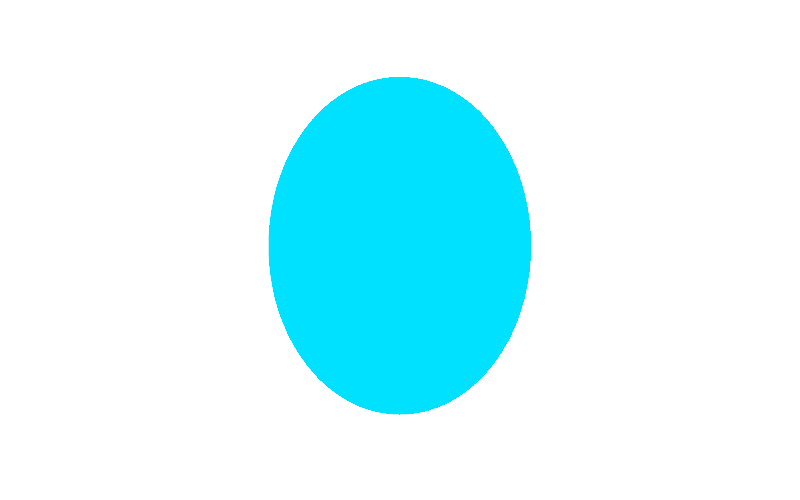
\includegraphics[height=1.5em]{ica3.png}}}$ CA3 inhibitory}
  & $20 \pm 7$                              & \citet{tukkerDistinct2013}
  & \multirow[t]{3}{*}{6.51}
  &                                         &
  & \multirow[t]{3}{*}{65.4\%} \\
  & $17 \pm 7$                              & \citet{laprayBehaviordependent2012}
  & & & & \\
  & $8.2 \pm 5.6$                           & \citet{leaoOLM2012}
  & & & & \\
\bottomrule
\end{tabular}}
\caption{%
  \textit{In vivo} firing rates and activation (the fraction of active cells) for each cell type, alongside model values.
  \textit{In vivo} firing rates are mean $\pm$ SD\@. \textsuperscript{max} maximum firing rate evoked by depolarizing current
  injection \textit{in vitro} (mean $\pm$ SEM for the HIPP cells). $\approx$ approximate value read from figure. Model firing rates are the mean over active cells and model activation the fraction of active cells; both are from
  the control network, except the immature granule cells (absent in the control), which are from the neurogenesis model at 50\%
  EC$\to$iGC excitability}
\label{tab:firing_rates}
\end{table}

%% =====================================================================
%% Figure S1 -- pattern separation resolved by input similarity
%% =====================================================================
\begin{figure}[H]
    \centering
    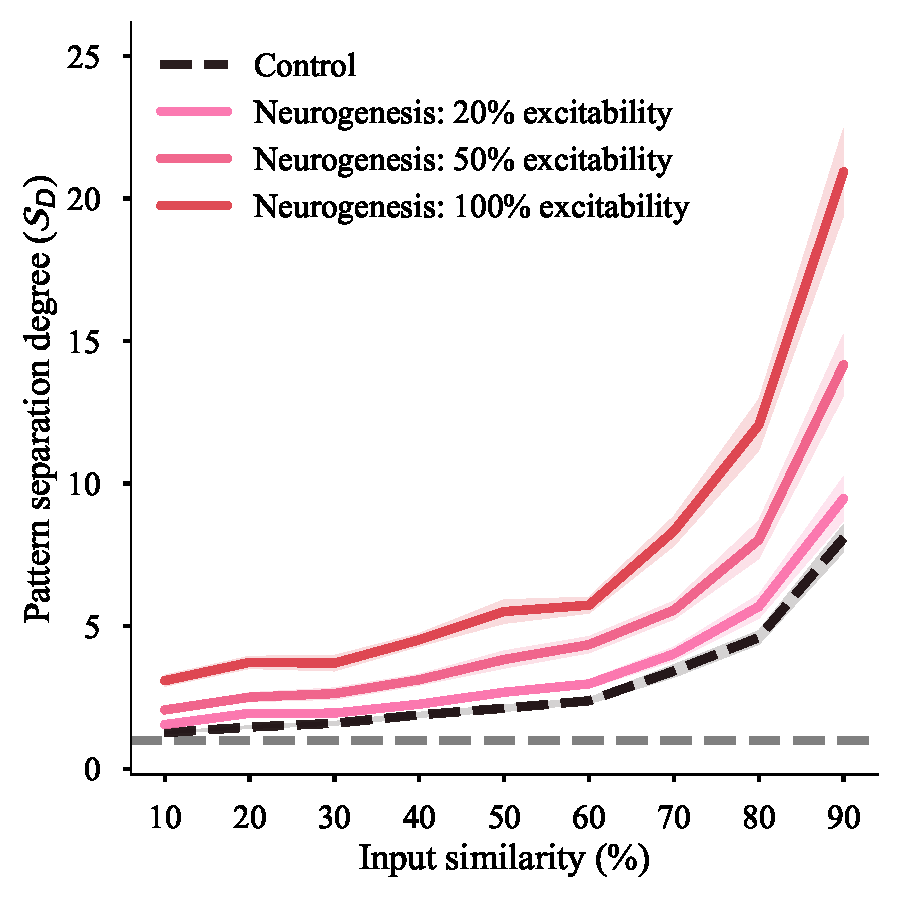
\includegraphics[width=0.7\linewidth]{supplementary_figures/pattern_separation.pdf}
    \caption{Pattern separation of the mature granule cells resolved by input similarity. Each curve shows the pattern separation
        degree $\mathcal{S}_D$ of the mGC population as a function of the similarity between the input patterns, for the control
        network without neurogenesis (black dashed line) and for neurogenesis networks at representative EC$\to$iGC excitability
        levels. Each point is the mean over the 30 pattern sets and the shaded band shows the standard error of the mean. The grey
        dashed line marks $\mathcal{S}_D = 1$, above which the output patterns are more distinct than their inputs. Separation is
        strongest for the most similar (most overlapping) inputs, and every neurogenesis network separates better than the control
        across the whole similarity range}\label{fig:pattern_separation_similarity}
\end{figure}

%% =====================================================================
%% Figure S2 -- Hoyer sparsity (cross-validation of the Gini index)
%% =====================================================================
\begin{figure}[H]
    \centering
    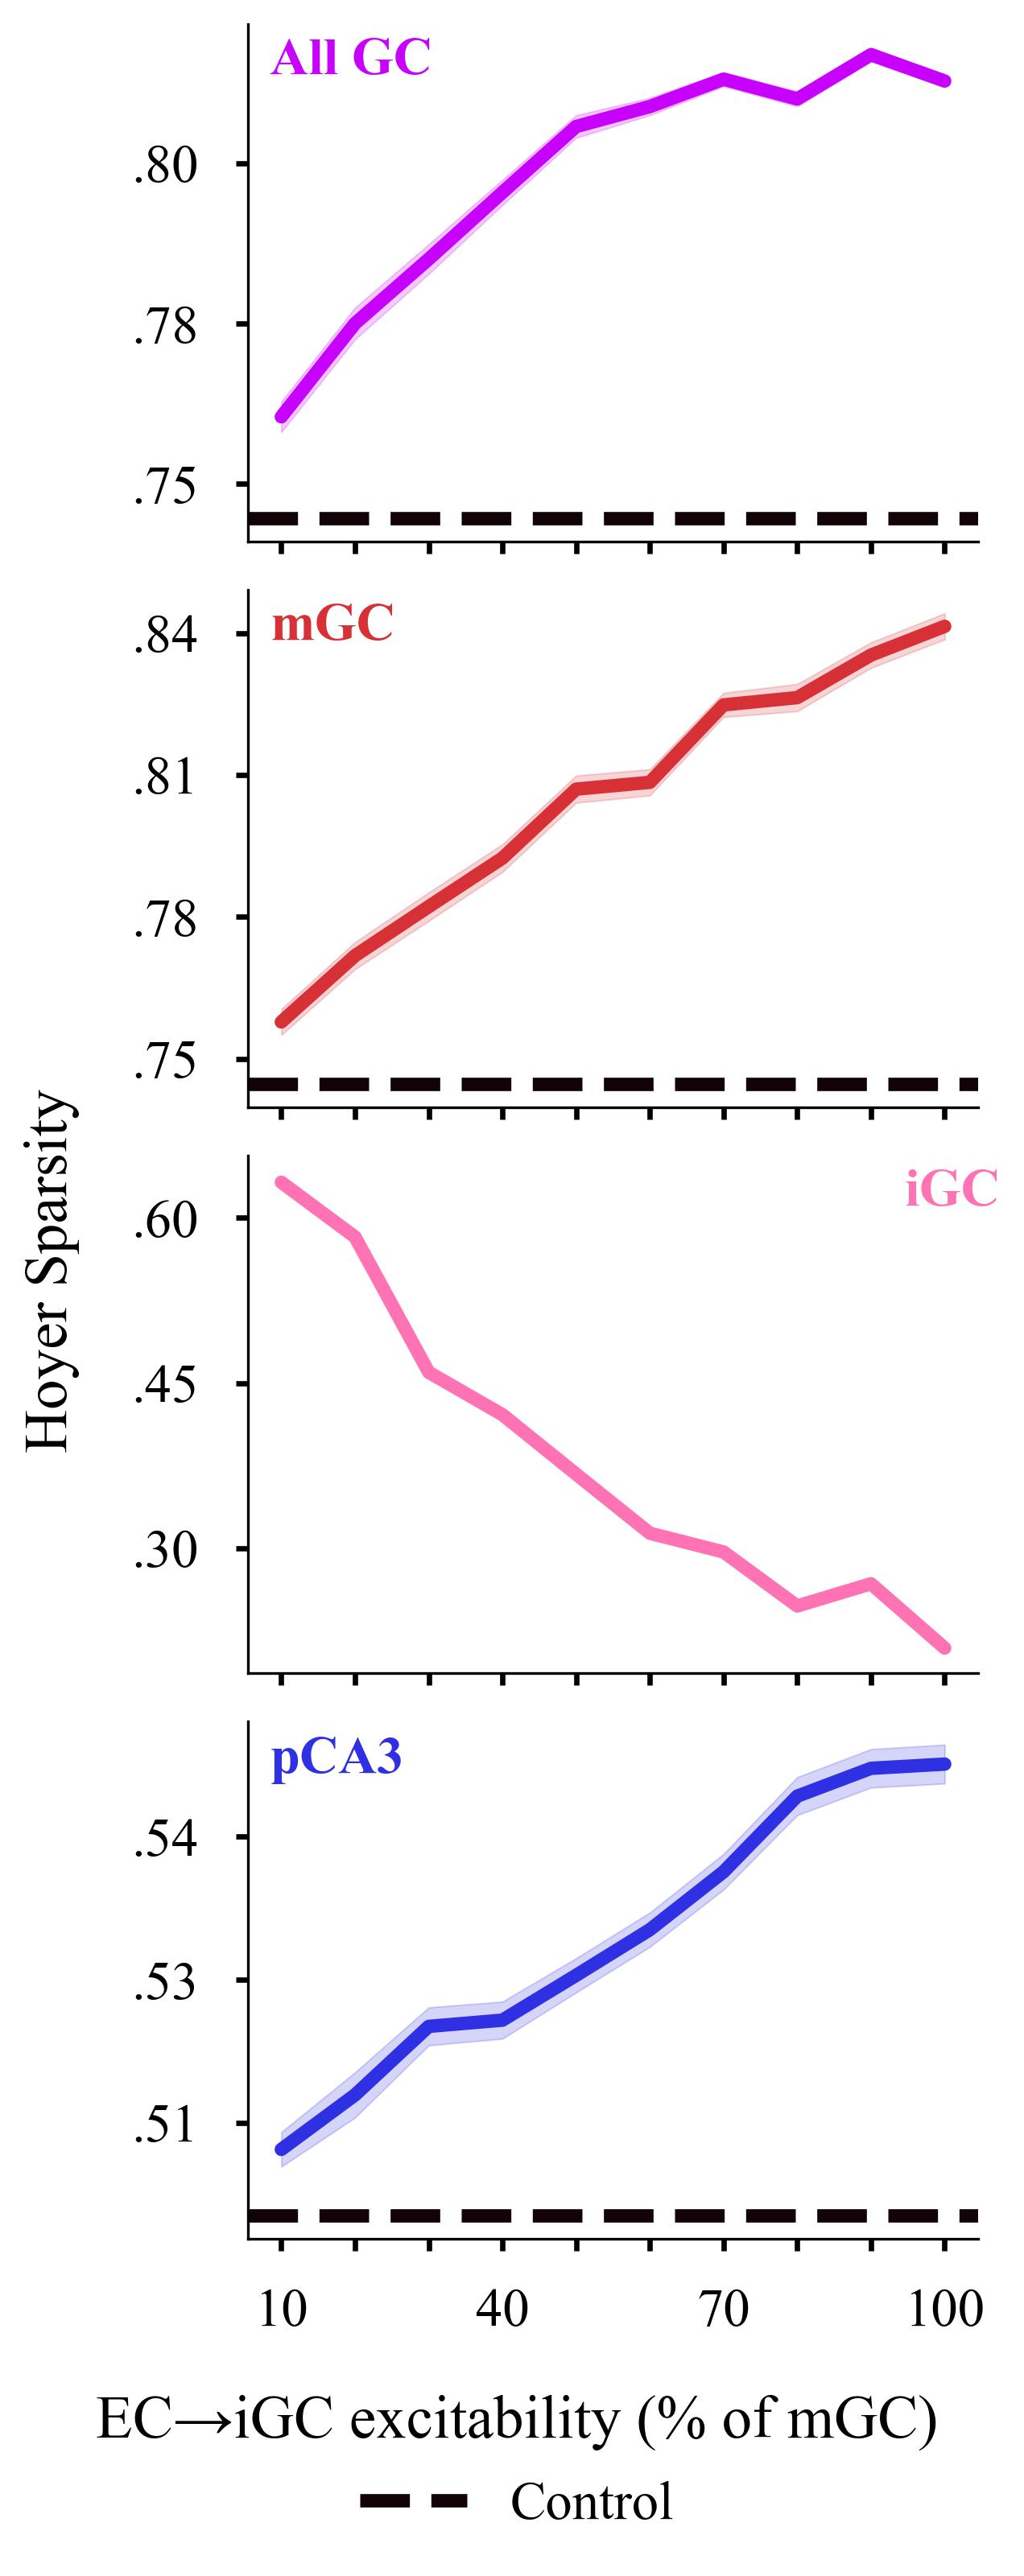
\includegraphics[width=0.42\linewidth]{supplementary_figures/sparsity_hoyer.jpg}
    \caption{Population sparsity measured with the Hoyer index, as a
        cross-validation of the Gini results reported in the main text. Each
        panel shows the Hoyer sparsity of one population, the whole
        granule-cell population (All GC), the mature granule cells (mGC), the
        immature granule cells (iGC) and the pyramidal CA3 cells (pCA3), as a
        function of the EC$\to$iGC excitability level; the shaded bands show the
        standard error of the mean and the dashed line marks the control network
        without neurogenesis (absent for the iGC panel, which has no counterpart
        in the control). As with the Gini index, the sparsity of the All GC, mGC
        and pCA3 populations rises with iGC excitability and stays above the
        control, whereas the iGC population becomes less
        sparse}\label{fig:sparsity_hoyer}
\end{figure}

%% =====================================================================
%% Figure S3 -- mGC orthogonalization degree
%% =====================================================================
\begin{figure}[H]
    \centering
    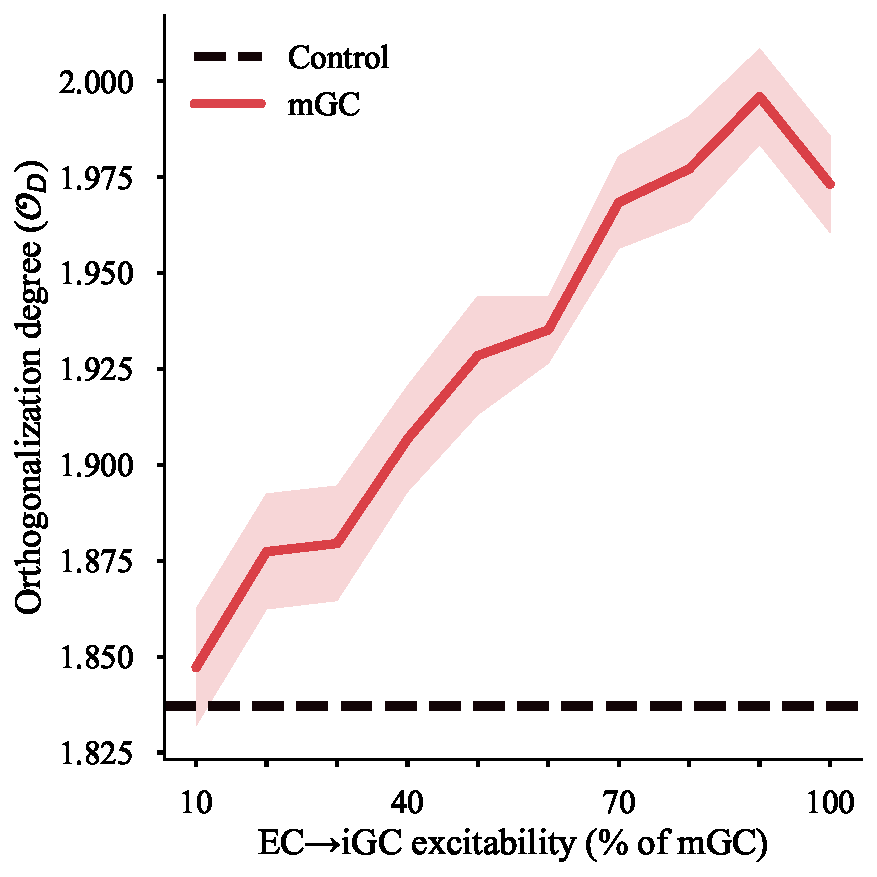
\includegraphics[width=0.6\linewidth]{supplementary_figures/mgc_orthogonalization.pdf}
    \caption{Orthogonalization of the mature granule-cell output as a function of EC$\to$iGC excitability. The curve shows the
        orthogonalization degree $\mathcal{O}_D$ of the mGC population, taken as the ratio of the output to the input
        orthogonalization ($O^{(out)}/O^{(in)}$); the shaded band shows the standard error of the mean and the dashed line marks
        the control network without neurogenesis. The orthogonalization rises with iGC excitability, indicating that the mGC
        outputs become increasingly decorrelated as neurogenesis increases, beyond what the reduction in the number of active
        cells alone would produce}\label{fig:mgc_orthogonalization}
\end{figure}

%% =====================================================================
%% Figure S4 -- pre/post Gini per excitability level (Wilcoxon)
%% =====================================================================
\clearpage
\begin{figure}[H]
    \centering
    \begin{subfigure}{0.30\linewidth}\centering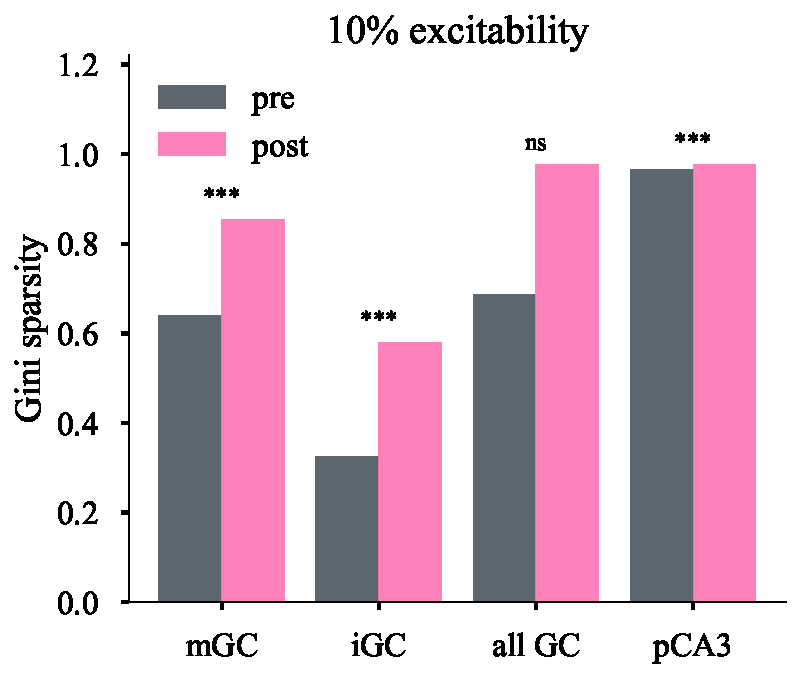
\includegraphics[width=\linewidth]{supplementary_figures/opto_sparsity_neurogenesis_0.1.pdf}\end{subfigure}\hfill
    \begin{subfigure}{0.30\linewidth}\centering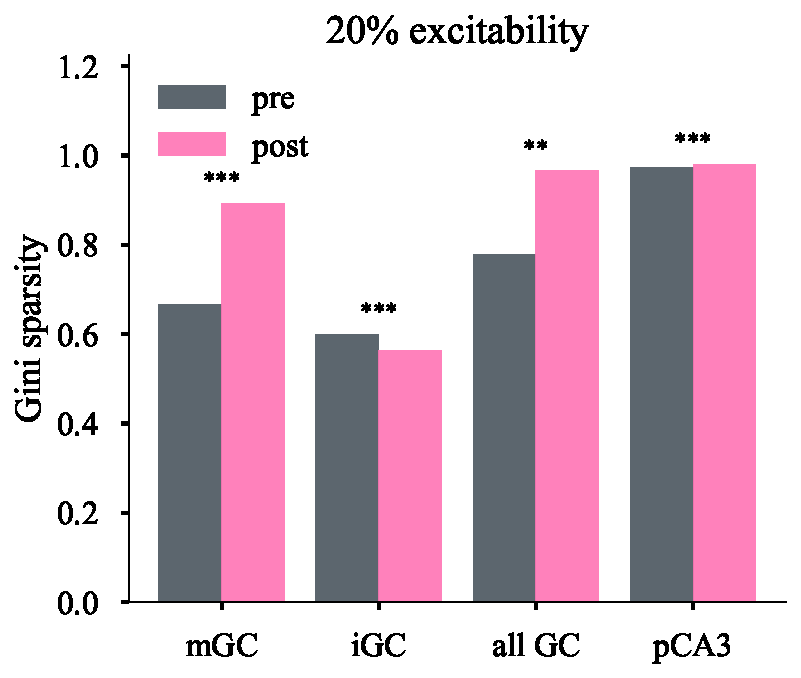
\includegraphics[width=\linewidth]{supplementary_figures/opto_sparsity_neurogenesis_0.2.pdf}\end{subfigure}\hfill
    \begin{subfigure}{0.30\linewidth}\centering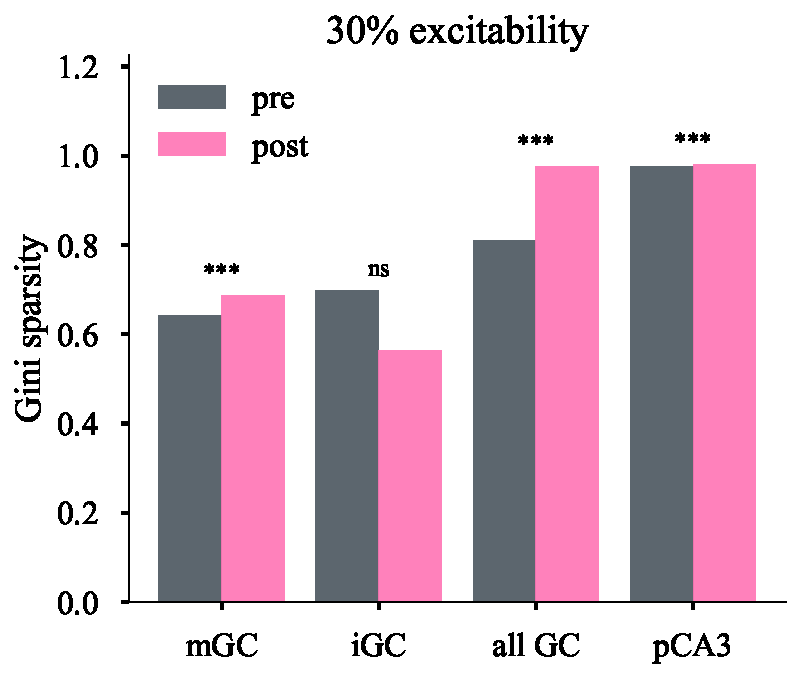
\includegraphics[width=\linewidth]{supplementary_figures/opto_sparsity_neurogenesis_0.3.pdf}\end{subfigure}

    \medskip

    \begin{subfigure}{0.30\linewidth}\centering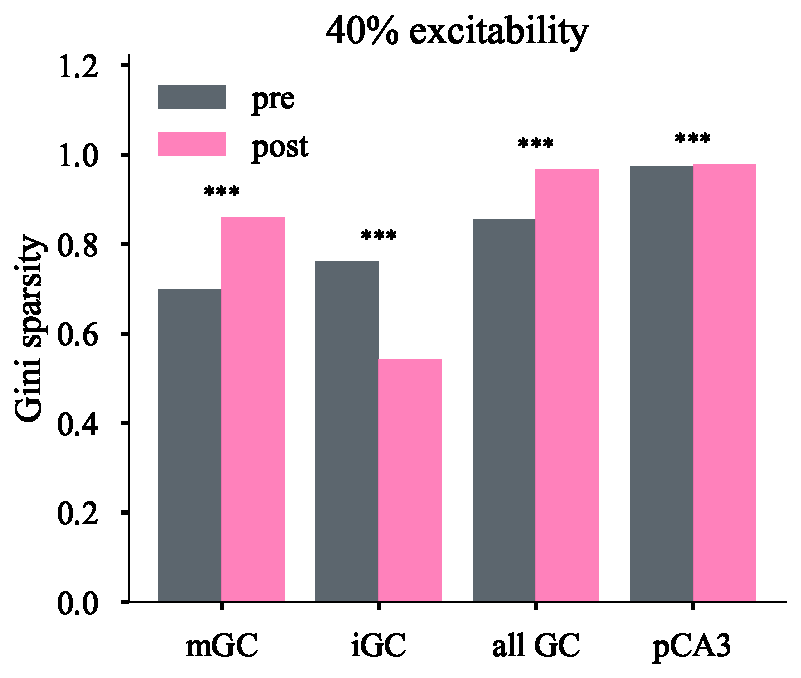
\includegraphics[width=\linewidth]{supplementary_figures/opto_sparsity_neurogenesis_0.4.pdf}\end{subfigure}\hfill
    \begin{subfigure}{0.30\linewidth}\centering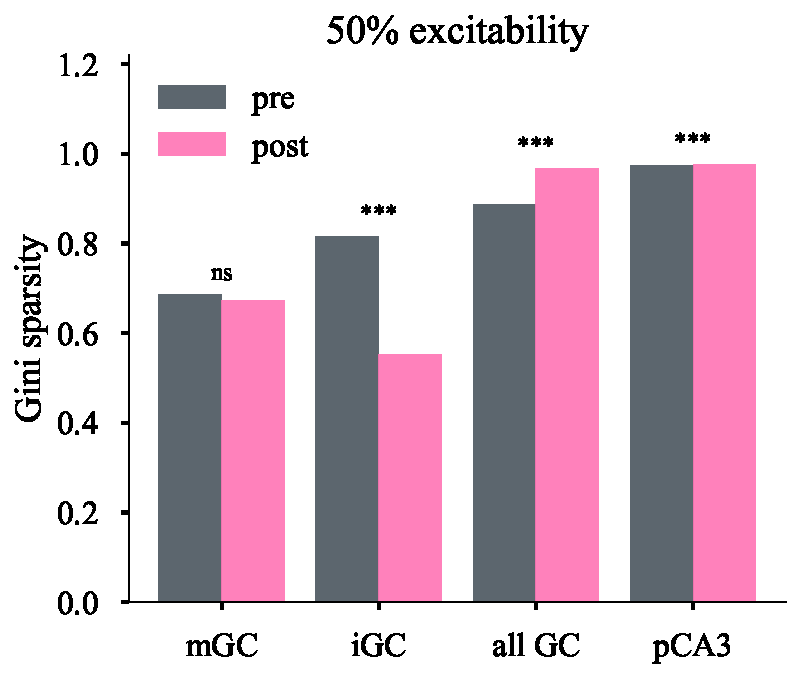
\includegraphics[width=\linewidth]{supplementary_figures/opto_sparsity_neurogenesis_0.5.pdf}\end{subfigure}\hfill
    \begin{subfigure}{0.30\linewidth}\centering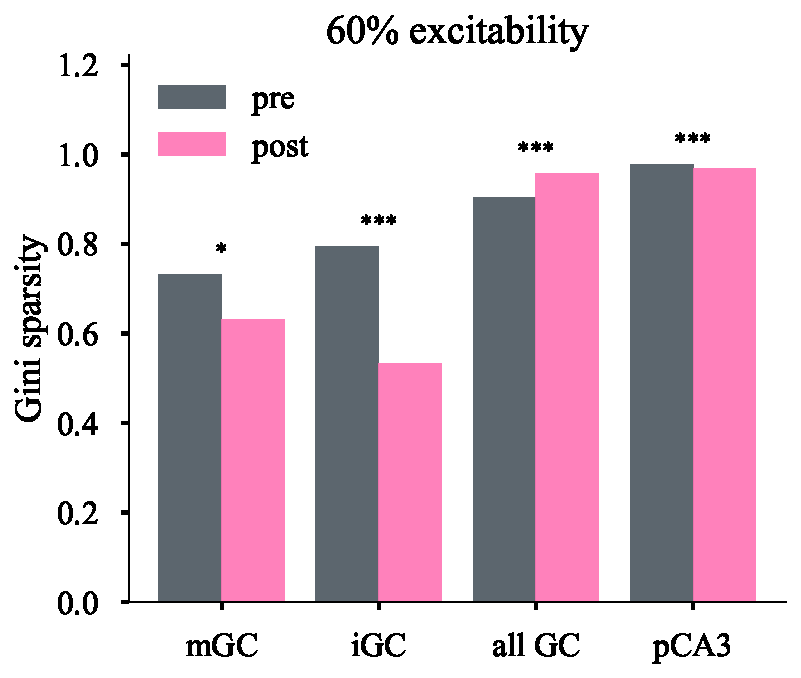
\includegraphics[width=\linewidth]{supplementary_figures/opto_sparsity_neurogenesis_0.6.pdf}\end{subfigure}

    \medskip

    \begin{subfigure}{0.30\linewidth}\centering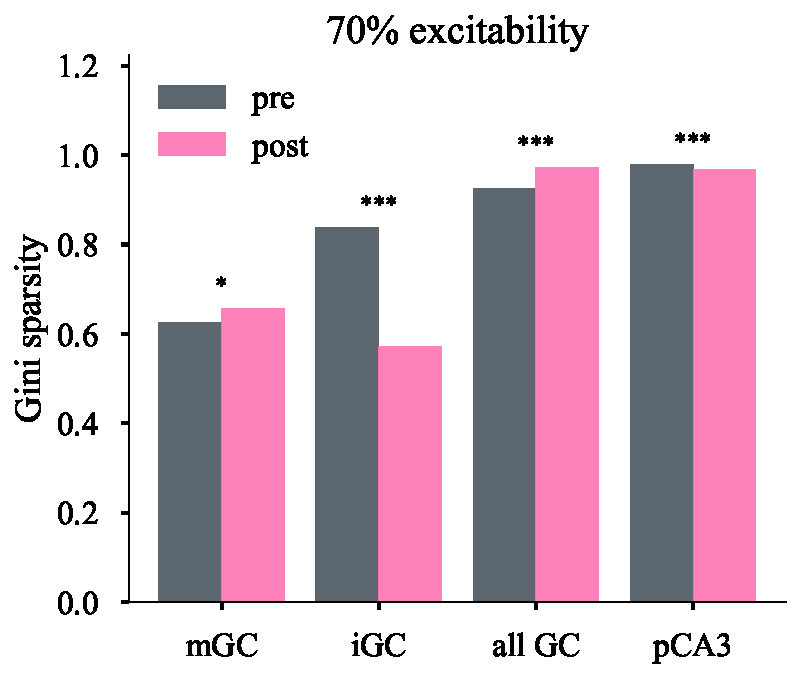
\includegraphics[width=\linewidth]{supplementary_figures/opto_sparsity_neurogenesis_0.7.pdf}\end{subfigure}\hfill
    \begin{subfigure}{0.30\linewidth}\centering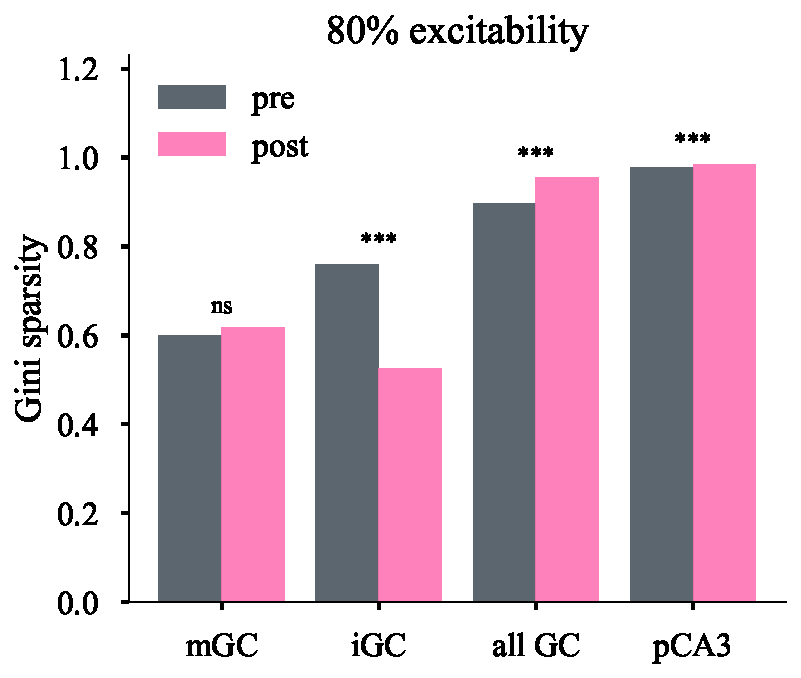
\includegraphics[width=\linewidth]{supplementary_figures/opto_sparsity_neurogenesis_0.8.pdf}\end{subfigure}\hfill
    \begin{subfigure}{0.30\linewidth}\centering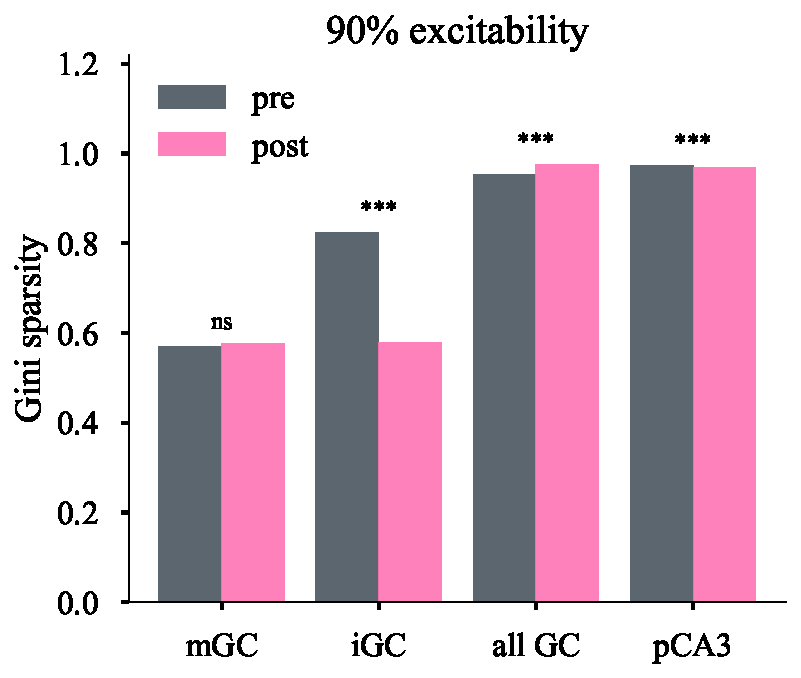
\includegraphics[width=\linewidth]{supplementary_figures/opto_sparsity_neurogenesis_0.9.pdf}\end{subfigure}

    \medskip

    \begin{subfigure}{0.30\linewidth}\centering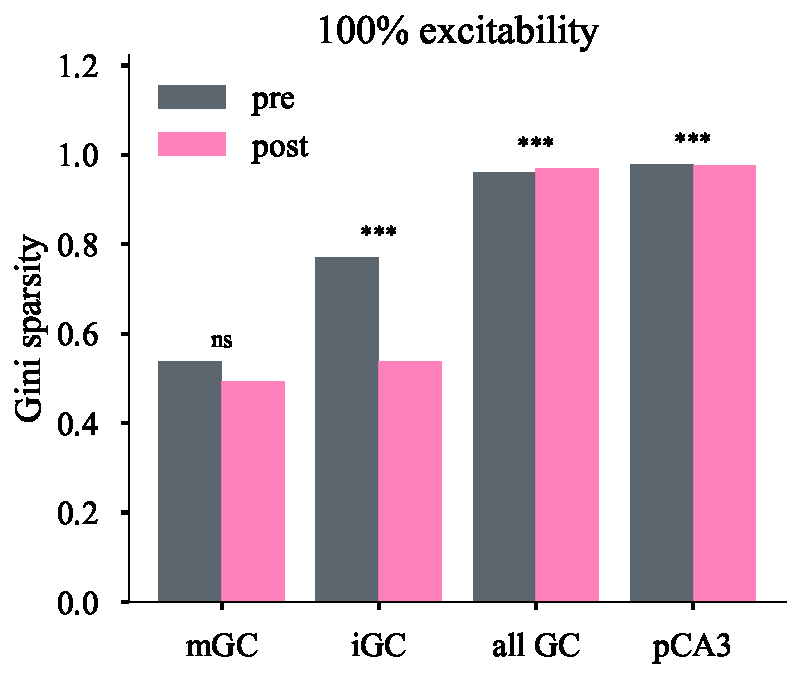
\includegraphics[width=\linewidth]{supplementary_figures/opto_sparsity_neurogenesis_1.0.pdf}\end{subfigure}\hfill
    \begin{subfigure}{0.30\linewidth}\end{subfigure}\hfill
    \begin{subfigure}{0.30\linewidth}\end{subfigure}

    \caption{Population sparsity (Gini index) immediately before and after direct iGC activation, for every EC$\to$iGC
        excitability level. Each panel corresponds to one excitability level (10\%--100\%, given in the panel title) and compares
        the Gini index of the mGC, iGC, combined granule-cell (all GC) and pCA3 populations in the \SI{50}{\milli\second} windows
        immediately before (pre) and after (post) the depolarizing pulse, pooled over all runs. Bars show the mean across runs.
        The result of the paired Wilcoxon signed-rank test between the pre and post values is indicated above each pair (ns, not
        significant; {*}~$p < 0.05$; {**}~$p < 0.01$; {***}~$p < 0.001$)}\label{fig:opto_sparsity}
\end{figure}

%% =====================================================================
%% Figure S5 -- post-pulse population rate and power spectrum per cell type
%% =====================================================================
\clearpage
\begin{figure}[H]
    \centering
    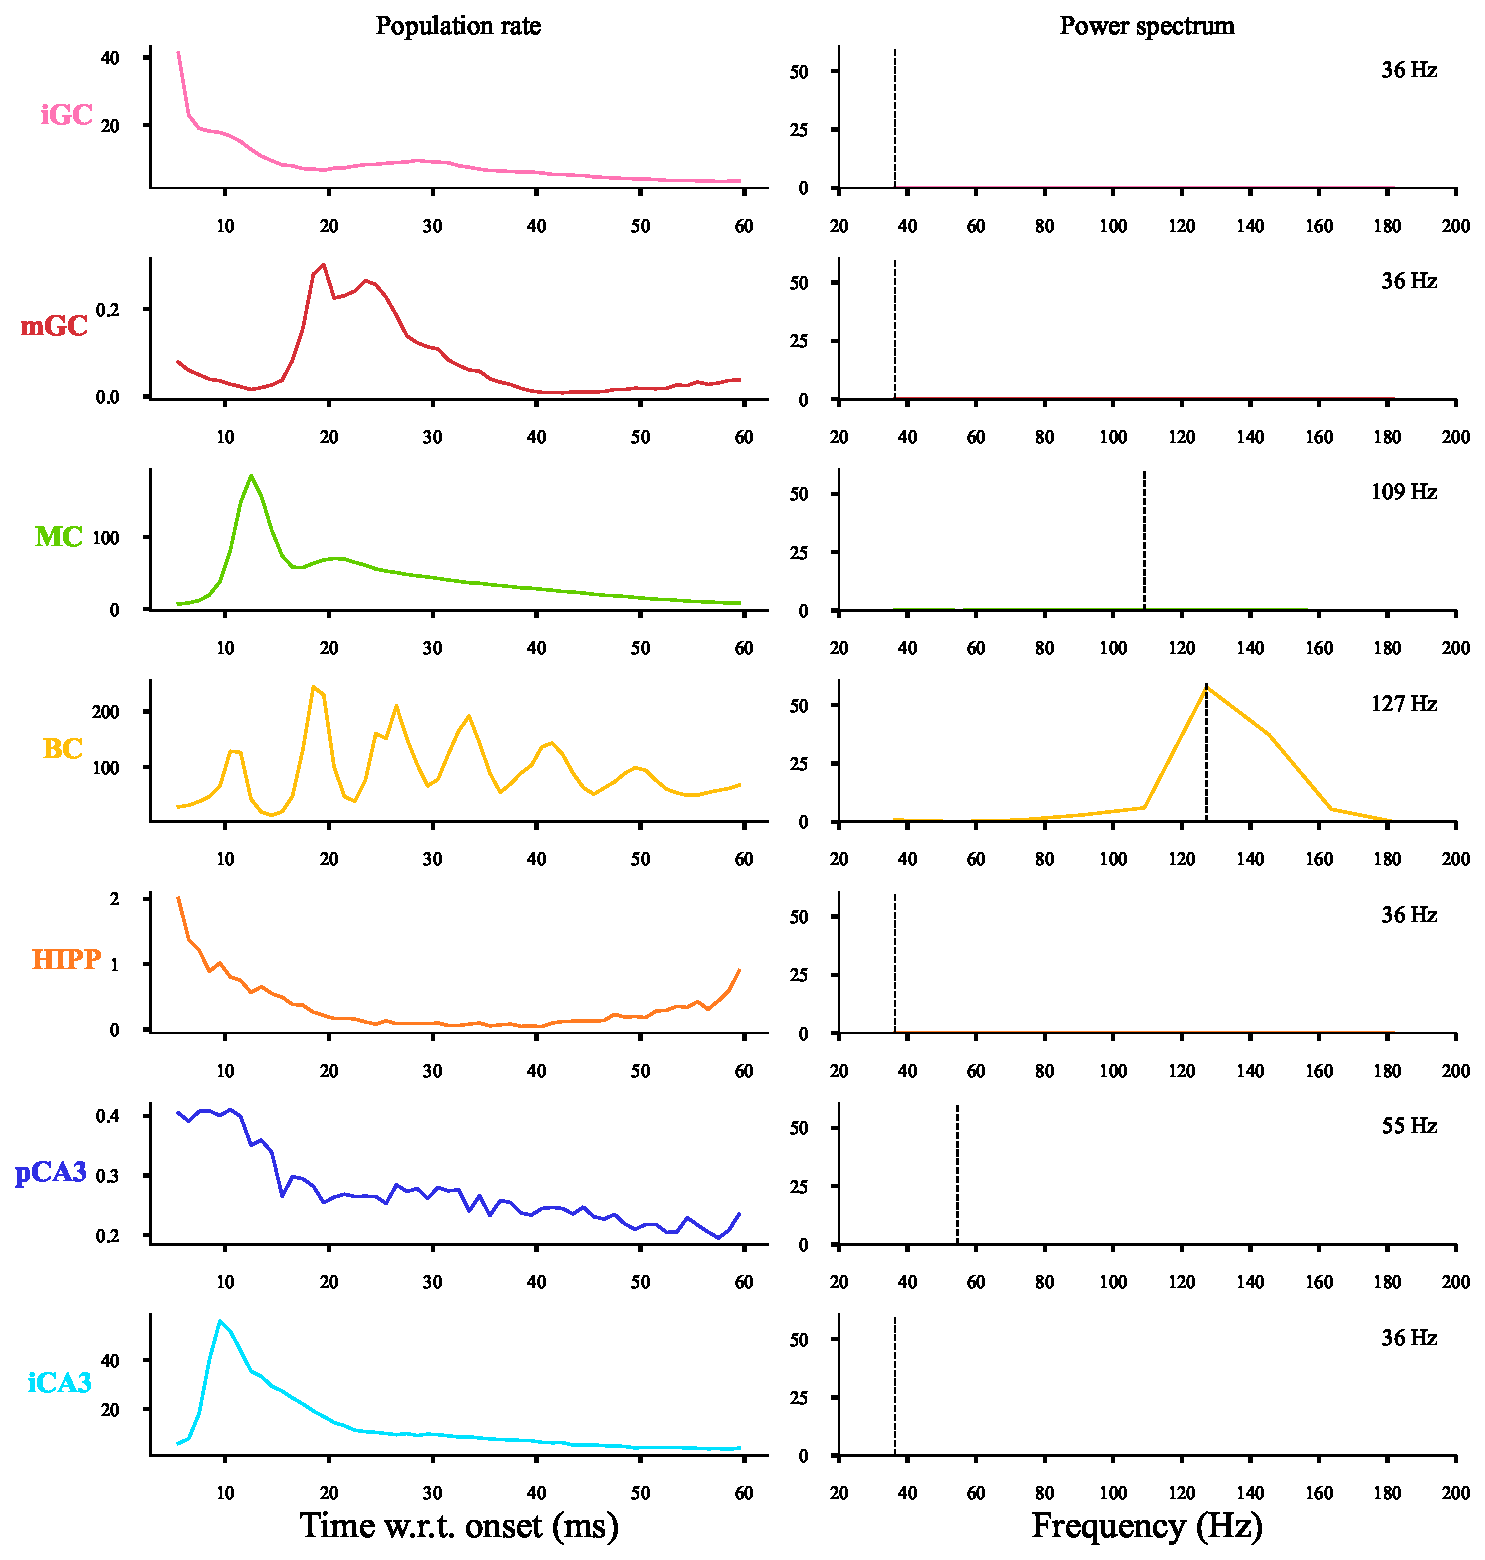
\includegraphics[width=0.85\linewidth]{supplementary_figures/frequency_pos_all.pdf}
    \caption{Rhythmicity of the post-pulse response of each population. Left column, population firing rate over the
        \SIrange{5}{60}{\milli\second} window following the onset of the depolarizing pulse delivered to half of the iGCs, pooled
        over all EC$\to$iGC excitability levels and all runs. Right column, power spectrum of the same signal after subtraction of
        a Gaussian-smoothed envelope, estimated by Welch's method over the \SIrange{20}{200}{\hertz} band; the dashed line and the
        label mark the peak frequency. Only the BCs show a spectral peak that stands out from the background of their own
        spectrum, at the frequency reported in the main text; the peak of the MCs carries a power close to the median of their
        band and the remaining populations peak at the lower edge of the band. The \SI{55}{\milli\second} analysis window sets the
        frequency resolution at \SI{18}{\hertz}, so the peak frequencies are accurate only to within one
        bin}\label{fig:frequency_spectra}
\end{figure}

\bibliographystyle{plainnat}
\bibliography{sn-bibliography}

\end{document}
